\chapter{Projektmanagement}
%Abhängigkeiten sollen in einem Schaubild veranschaulicht werden

\section{Arbeitspakte}
%Meilensteine sollen auf den Zeitplan verweisen und umgekehrt

%2.1 Klare Definition von Forschungszielen und Teilzielen
%Erste Meilenstein Prio 1
%Der erste Meilenstein ist es die Schnittstelle über den gRPC Server und Client soll in beide richtungen Daten übertragen.
%Die Thales Sensordaten von 4 Sensoren müssen über den gRPC Server vom Client abgefragt werden können. Zur Aufnahme Zeit aber mindestens alle 40ms. 

\begin{figure}[h]
    \centering
    \includegraphics[width=15cm, page=1]{images/Arbeitspakete und ihre Abhängigkeiten.pdf}
    \caption{Arbeitspakete und ihre Abhängigkeiten}
    \label{fig:Arbeitspakete}
\end{figure}
Innerhalb des ersten Hauptarbeitpakets liegt der Fokus auf der Umsetzung einer funktionsfähigen Schnittstelle zwischen dem gRPC Server und Client, um Daten in beiden Richtungen zu übertragen. \\
Ein zentrales Ziel ist es, Thales Sensordaten von insgesamt 4 Sensoren über den gRPC Server vom Client abrufen zu können. Die Datenabfrage sollte in der Lage sein, mit einer Aufnahmefrequenz von mindestens alle 40 Millisekunden durchgeführt zu werden.\\
%Über den gRPC Server sollen auch andere Parameter übertragen werden wie Lenkwinkel oder Geschwindigkeit einer im späteren verlauf erstellten AGVs.
Zusätzlich zu den Sensordaten sollen auch andere Parameter über den gRPC Server übertragen werden, wie beispielsweise der Lenkwinkel oder die Geschwindigkeit eines zukünftig erstellten AGVs. Diese Datenübertragung wird durch die CustumApi umgesetzt. Dieses Hauptarbeitpaket bildet einen wesentlichen Schritt, um die grundlegende Funktionalität des Projektes zu etablieren und legt den Grundstein für die weitere Entwicklung im Projektverlauf.\\
%Zweiter Meilenstein Prio 2
%Der zweite Meilenstein soll die Umsetzung der AGVs enthalten. Dazu muss die Fahrphysik erstellt werden. Es sollten mehrer Arten von Agvs entwickelt werden aber mindestens eins. Zunächsten sollen ein AGVs nach einem normalen Auto erstellt werden dann ein Gabelstapler also ein dreiRad und dannach eine Panzerrolle in dieser Reinfolge.
Das zweite Hauptarbeitpakets umfasst die Erstellung der Fahrphysik für die AGVs. Dies beinhaltet die Realisierung von realistischen Bewegungsabläufen und Steuerungsmechanismen, die den Charakter der jeweiligen AGV-Typen authentisch wiedergeben.\\
Innerhalb dieses Meilensteins ist die Entwicklung mehrerer Arten von AGVs geplant, wobei mindestens eine Variante umgesetzt wird. Zunächst muss ein Lenksystem entwicktelt werden, das die Vorderräder des AGVs korrekt steuert. Unter der Berücksichtigung der physikalischen Gesetzt der Lenkung und die Beziehung zwischen Lenkwinkel und Fahrzeugbewegung.\\
Die Umsetzung einer realistischen und kontrollierbaren Beschleunigungsmechanik ist ebenfalls ein Teil des Hauptarbeitpakets. Entwicklung eines Beschleunigungssystems, das die Bewegung des Fahrzeugs steuert und die Kraftübertragung auf die Antriebsräder regelt. Die Entwicklung von Lenksystem und Beschleunigung ist substanziell für die nächste Aufgabe.\\

Das AGV wird über ein Fahranweisungsscript gesteuert. Das Fahranweisungsscript wird Funktionen und Methoden zur Steuerung von Beschleunigung, Bremsung und Lenkung enthalten.\\

Im späteren Verlauf werden verschiedene AGVs entworfen, darunter ein AGV, das auf einem herkömmlichen Auto basiert, gefolgt von einem dreirädrigen Gabelstapler und schließlich einer Panzerrolle.\\
%Die Steuerung oder Fahranweisung soll über ein Script in Unity laufen welches sagt geschwindigkeit/Beschleunigung gibt und Lenkeinschlag der steuerachse
Die erfolgreiche Umsetzung dieses Meilensteins wird die Basis für die funktionale und realistische Integration der AGVs in das Forschungsprojekt legen. Durch die Entwicklungsarbeit im zweiten Meilenstein wird die Grundlage für weiterführende Tests und Analysen der AGVs geschaffen, die zur Erreichung der gesamten Projekts beitragen.\\

%Dritter Meilenstein Prio 3 Dritter Meilenstein: Erfassung des AGV-Bremswegs als Polygonzug
%Im Dritten Meilenstein solle ein Polygonzug erhalten werden der den Bremsweg des AGVs wiederspielt. Er kann dierkt an erhalten werden jedoch muss noch überprüft werden ob es möglich ist ihn zu übertragen oder ob einfach die die länge des bremsschlauchs und darus mit dem lenkeinschlag der Bremsweg darstellt wird.


\begin{figure}[h]
    \centering
    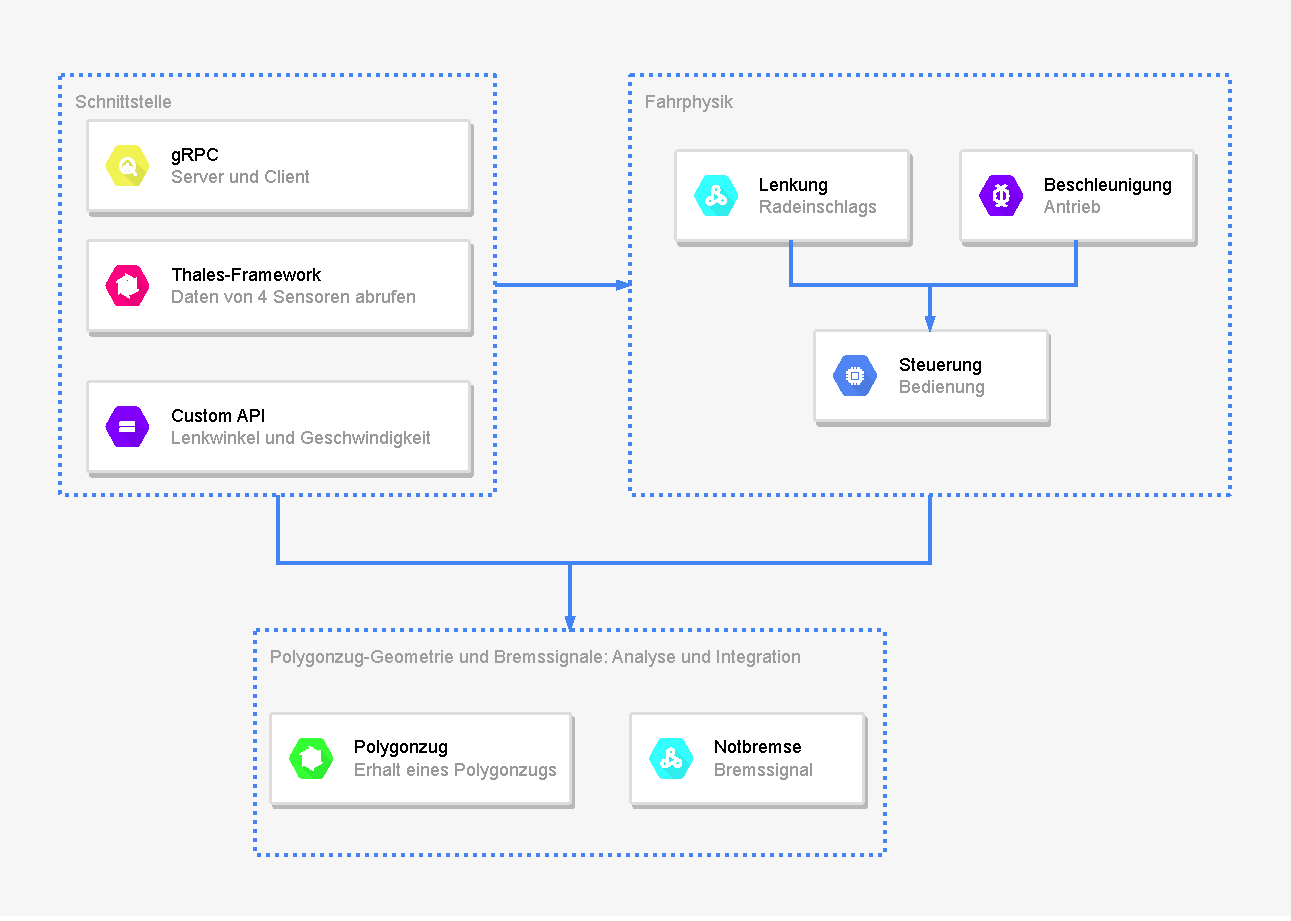
\includegraphics[width=15cm, page=1]{images/Poly.pdf}
    \caption{Arbeitspakete}
    \label{fig:Arbeitspaket}
\end{figure}

Innerhalb des Dritten Arbeitspakets ist das Hauptziel der eines Polygonzugs. Der Polygonzug soll außerhalb von Unity mit Geschwindigkeit und Einschlagwinkel des AGVs berechnet werden. Dieser Polygonzug soll den Verlauf des Bremsvorgangs in einer geometrischen Darstellung wiedergeben.\newline
Nach dem Erhalt des Polygonzugs muss überprüft werden, ob dieser direkt auf das AGV-Modell übertragen werden kann. Es ist von Bedeutung zu ermitteln, ob die Daten des Polygonzugs in das Simulationssystem eingeführt werden können, um eine korrekte Darstellung des Bremsverhaltens zu ermöglichen.\newline
Der Polygonzug wird außerhalb des Projekts berechnet und erstellt. Der DSM Host erhält die Scanner Daten, den Lenkeinschlag und die Geschwindigkeit des AGVs. Der Algorithmus zur Berechnung des Schutzfeldes und Polygonzugs, wird im DSM Host entwickelt.
%Falls eine direkte Übertragung des Polygonzugs nicht möglich ist, wird eine alternative Methode in Betracht gezogen. Hierbei wird die Länge des Bremsschlauchs in Verbindung mit dem Lenkeinschlag genutzt, um den Bremsweg auf eine plausible Weise darzustellen.\newline
%Die erfolgreiche Erfassung des AGV-Bremswegs als Polygonzug oder über alternative Darstellungsformen wird eine wichtige Grundlage für die Simulation des Bremsverhaltens in späteren Forschungsphasen bilden. Dieser Meilenstein trägt dazu bei, das Verhalten des AGVs unter verschiedenen Bedingungen besser zu verstehen und die Gesamtfunktionalität des Modells zu verbessern.\\

%Der vierte Meilenstein soll dafür sorgen das das Agv durch ein Siganl vom gRPC Client abbremst
Im Rahmen Dritten Arbeitspakets wird das Ziel verfolgt, die Signalübertragung vom gRPC-Client zum AGV zu implementieren. Das Signal soll die Abbremsung des AGVs auslösen, wenn es empfangen wird.\\
Es ist von entscheidender Bedeutung, die Steuerungsfunktion im AGV zu konfigurieren, damit sie auf das empfangene Signal reagiert und die notwendigen Maßnahmen zur Abbremsung einleitet.\\
Die erfolgreiche Umsetzung dieses Meilensteins wird die Fähigkeit des AGVs zur externen Steuerung und zur Initiierung einer Abbremsung über das gRPC-Client-Signal demonstrieren. Diese Funktionalität kann im weiteren Verlauf der Forschungsarbeit dazu verwendet werden, verschiedene Szenarien und Anwendungen zu testen, bei denen eine externe Steuerung des AGVs erforderlich ist.
Der DSM Host erhält die Scanner Daten, den Lenkeinschlag und die Geschwindigkeit des AGVs. Der Algorithmus zur Berechnung des Schutzfeldes, wird im DSM Host entwickelt. Der Host sendet auch das Bremssignal, die Entwicklung liegt außerhalb des zeitlichen Rahemen diese Projektes, weshalb das Bremssignal nur Testweise über den Client gesendet wird.\\
%2.2 Identifikation von wichtigen Meilensteinen im Forschungsprozess

%2.3 Unterteilung des Projekts in überschaubare Etappen
\section{Zeitplan}

\begin{figure}[h]
    \centering
    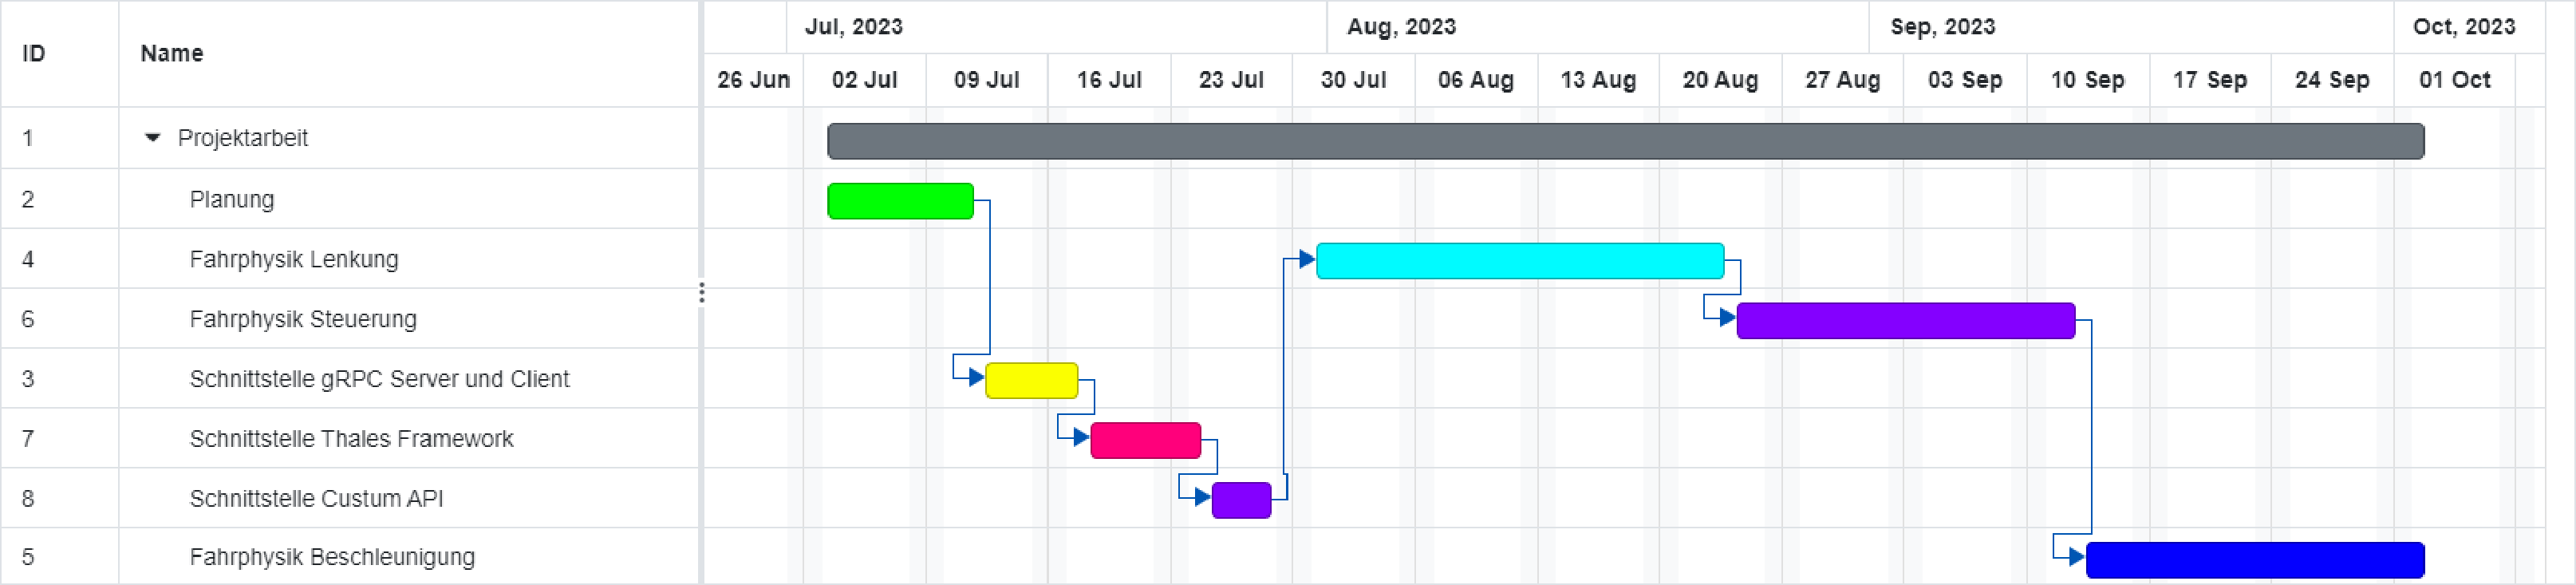
\includegraphics[width=18cm, page=1]{images/Zeitplan (3).pdf}
    \caption{Zeitplan}
    \label{Zeitplan}
\end{figure}
%Erstellung eines Zeitplans
%3.1 Festlegung von Start- und Enddatum des Projekts
Das Projekt startet am 3. Juli und die Abgabe der schriftlichen Projektarbeit ist am 21. September. Nach der Berücksichtungen der Abwesenheiten umfasst das Projekt 35 Arbeitstage.

%3.2 Strukturierung des Zeitplans nach Etappen und Meilensteinen
Die ausführliche Vorbereitung und Planung sind entscheidend, um die genauen Anforderungen und Ziele des Projekts zu klären, die Arbeitsschritte detailliert aufzuschlüsseln und die benötigten Ressourcen zu definieren. Die Vorbereitung und Planung wird auf 5 Tage geschätzt.\\
%3.3 Berücksichtigung von Pufferzeiten für unvorhergesehene Verzögerungen
Implementierung der gRPC-Server-Client-Schnittstelle erstreckt sich über zehn Tage, um sicherzustellen, dass die bidirektionale Datenübertragung zwischen dem Server und dem Client erfolgreich ermöglicht wird.\\

Die Umsetzung der AGVs dauert insgesamt zehn Tage. In zunächst wird die Fahrphysik für verschiedene AGV-Typen entwickelt, beginnend mit einem AGV, das sich wie ein herkömmliches Auto verhält. Die Bewegungsabläufe und Steuerung werden getestet und optimiert.\\

Die anderen Aufgaben können Aufgrund der Abhängigkeiten zu anderen Teilen des DSM Projekts und zugroßem Umfang nicht in den Zeitplan geschreiben werden.
%Gantt-Diagramme und Visualisierung
%4.1 Verwendung von Gantt-Diagrammen zur grafischen Darstellung des Zeitplans
%4.2 Einfache Veranschaulichung von Aufgaben, Dauer und zeitlichen Abhängigkeiten

       
%Abhängigkeiten und Priorisierung
%6.1 Erkennen von Aufgabenabhängigkeiten und Verknüpfungen
%6.2 Priorisierung von Aufgaben basierend auf ihrer Relevanz und Abhängigkeit

%Überwachung und Anpassung des Zeitplans
%7.1 Regelmäßige Überprüfung des Fortschritts im Vergleich zum Zeitplan
%7.2 Identifizierung von Abweichungen und Verzögerungen
%7.3 Anpassung des Zeitplans bei Bedarf unter Berücksichtigung der Gesamtziele


\section{Risikoanalyse}

Im Rahmen des Projekts wurden potenzielle Risiken identifiziert, die während der Umsetzung der Meilensteine und des 35-tägigen Zeitplans auftreten könnten. Diese Risiken wurden analysiert und bewertet, um angemessene Maßnahmen zur Risikobewältigung zu identifizieren.\\

\begin{figure}[htp]
    \centering
    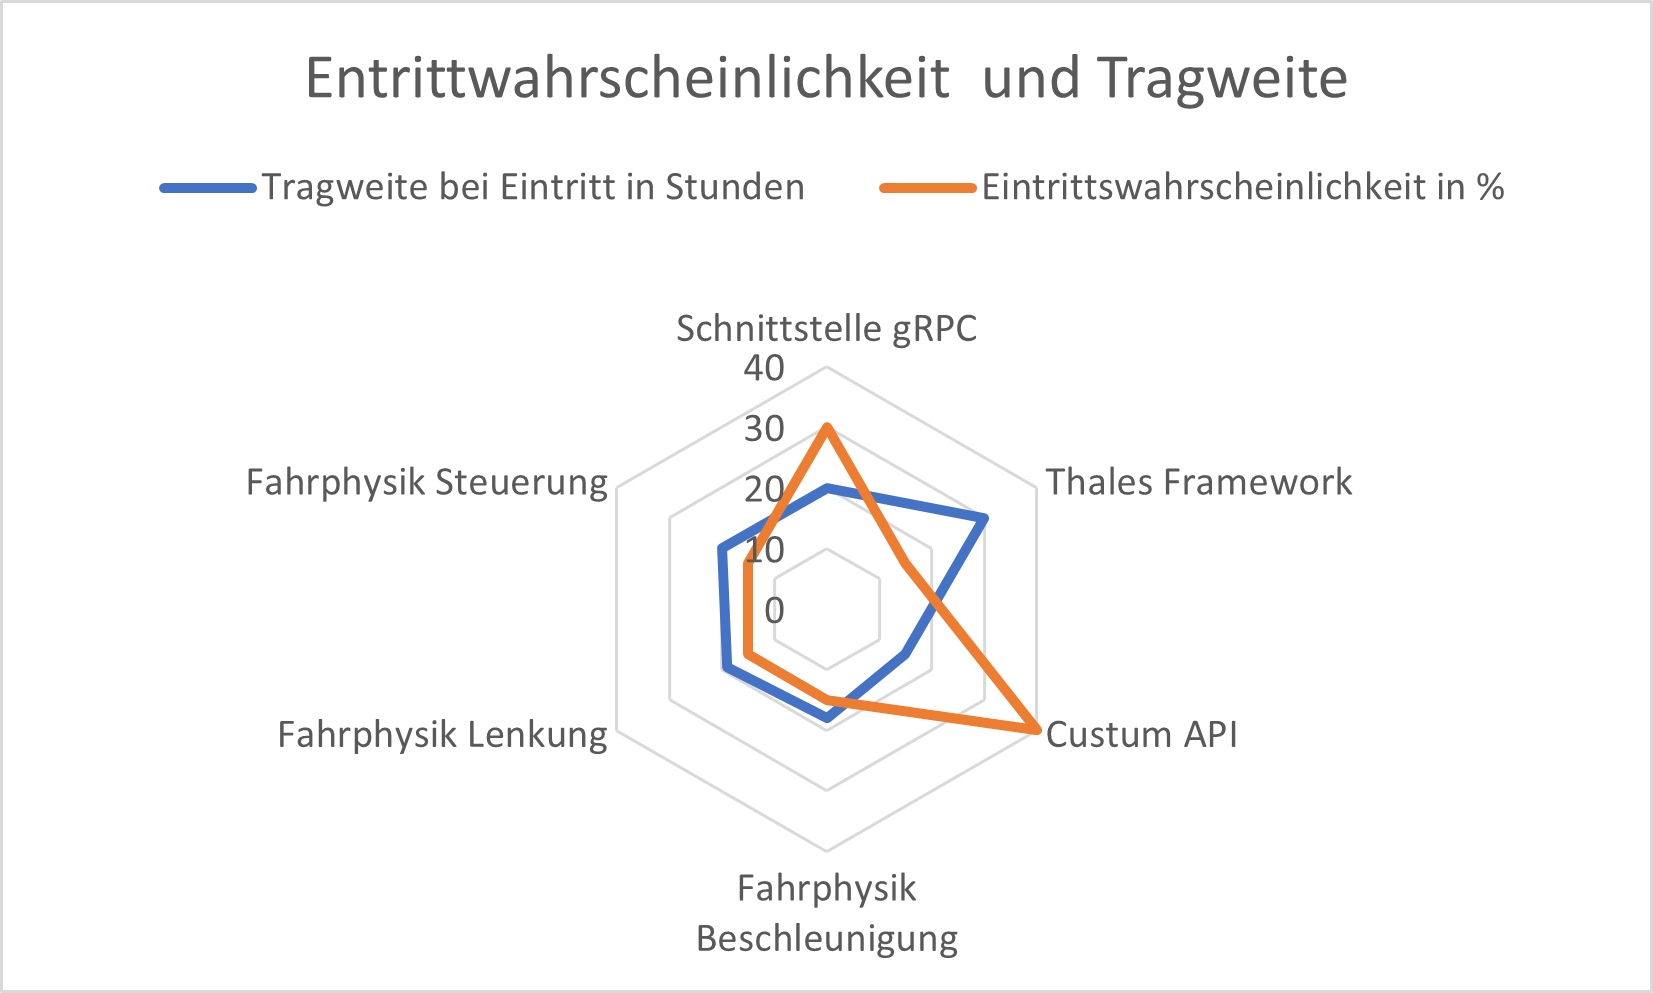
\includegraphics[width=(\textwidth)]{images/Tragweite.png}
    \caption{Eintrittswahrscheinlichkeit und Tragweite}
    \label{fig:Eintrittswahrscheinlichkeit}
\end{figure}

Ein hoch bewertetes Risiko besteht in technischen Herausforderungen bei der Implementierung der gRPC-Server-Client-Schnittstelle. Die Eintrittswahrscheinlichkeit wird als mittel eingestuft, aber die Auswirkungen könnten hoch sein, da dies die Grundlage für die Kommunikation im Projekt bildet. Ähnlich verhält es sich mit dem Risiko unvorhergesehener Schwierigkeiten bei der Signalübertragung für die externe Abbremsung. Hierbei könnte die Eintrittswahrscheinlichkeit mittel sein, aber die Auswirkungen wären hoch, da die externe Steuerung des AGVs beeinträchtigt werden könnte.\\

Die Umsetzung der AGV-Typen birgt das Risiko von Schwierigkeiten bei der Erstellung der Fahrphysik, da die Eintrittswahrscheinlichkeit als hoch eingeschätzt wird und die Auswirkungen mittel sein könnten. Zudem besteht die Gefahr von zeitlichen Verzögerungen bei der Umsetzung der AGV-Typen, da eine mittlere Eintrittswahrscheinlichkeit und mittlere Auswirkungen gegeben sind.\\

In Bezug auf den dritten Meilenstein, die Erfassung des Bremsweg-Polygonzugs, besteht das Risiko technischer Inkompatibilität bei der Übertragung, obwohl die Eintrittswahrscheinlichkeit niedrig ist, könnten die Auswirkungen mittel sein. Zusätzlich könnte das Risiko bestehen, dass sich die Anforderungen an den Bremsweg ändern, was jedoch als gering eingeschätzt wird.\\

Die mögliche Fehlkommunikation zwischen dem gRPC-Server und dem Client sowie unerwartete Schwierigkeiten bei der Konfiguration der Steuerungsfunktion für die externe Abbremsung könnten sich als hohe Risiken mit mittleren Auswirkungen erweisen.\\

Ein weiteres bedeutendes Risiko betrifft die mangelnde Verfügbarkeit von Ressourcen wie Hardware oder Software während des gesamten Projekts. Hierbei wird eine hohe Eintrittswahrscheinlichkeit angenommen, verbunden mit hohen Auswirkungen auf den Projektfortschritt.\\

Die Risikoanalyse zeigt auf, dass eine gründliche Planung und regelmäßige Überwachung der Projektschritte unerlässlich ist, um auf mögliche Risiken rechtzeitig reagieren zu können. Es empfiehlt sich, für jedes identifizierte Risiko geeignete Maßnahmen zur Risikominderung und -bewältigung zu entwickeln.\\


\begin{figure}[htbp]
    \centering
    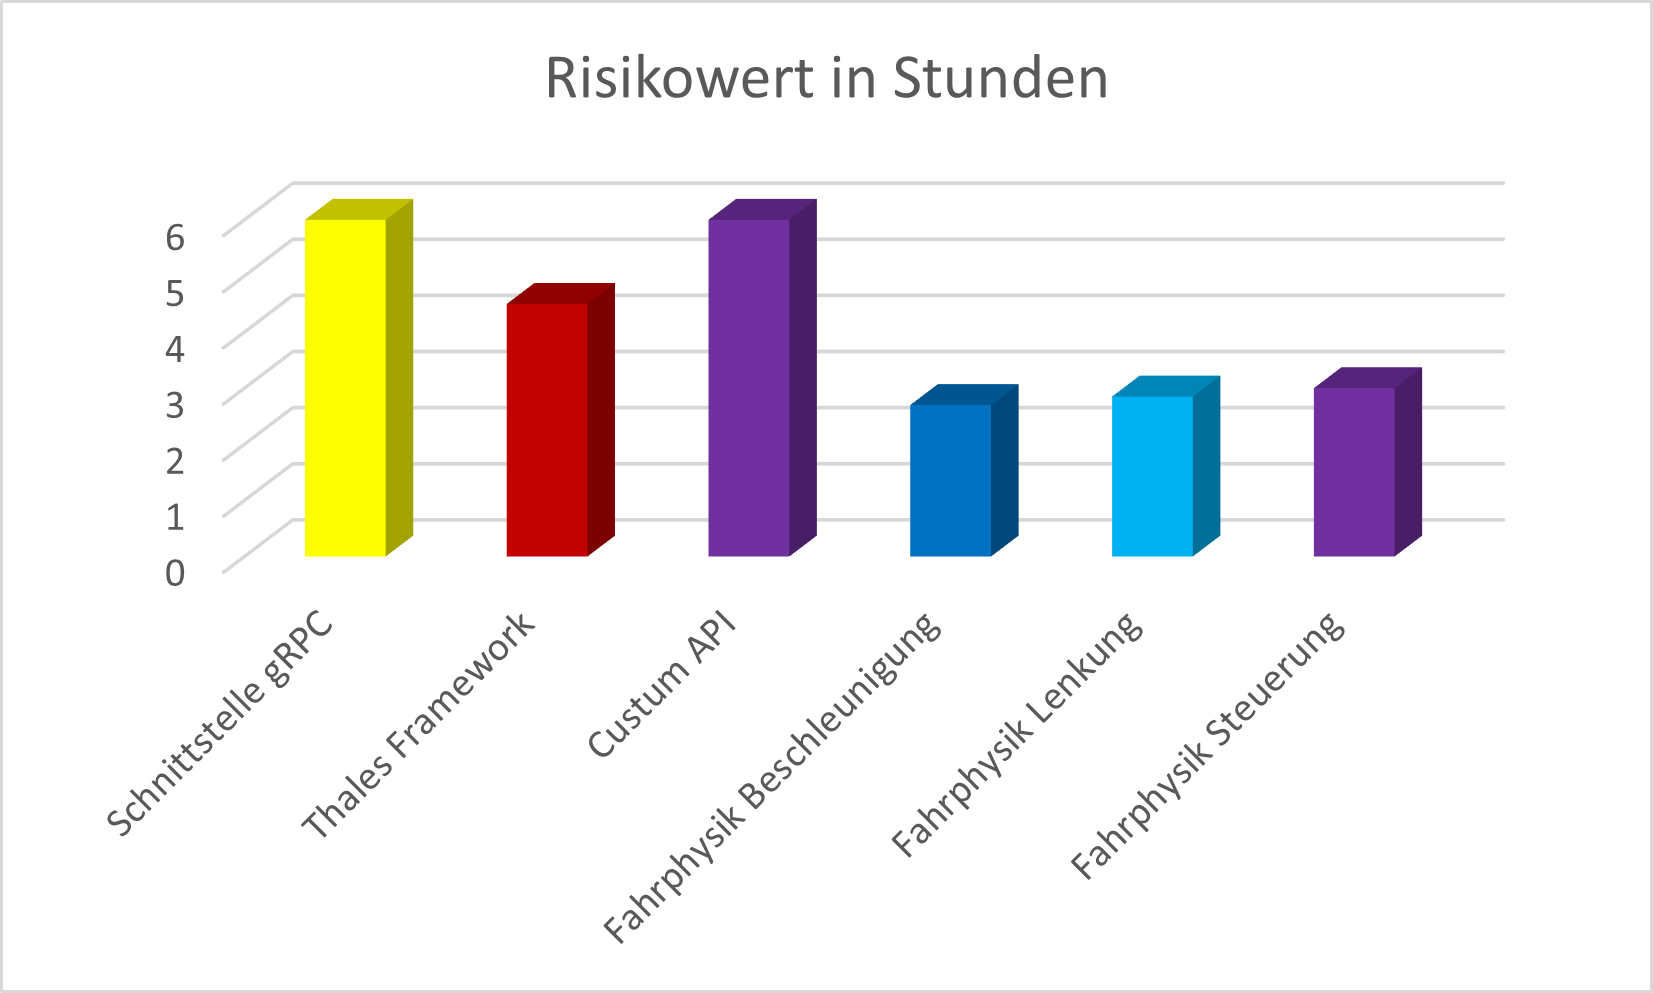
\includegraphics[width=(\textwidth)/2]{images/Risikowert.png}
    \caption{Risikowert in Stunden}
    \label{fig:Risikowert in Stunden}
\end{figure}

Die Berechnung des Risikowerts in einer Risikoanalyse erfolgt durch die Kombination von Eintrittswahrscheinlichkeit und Auswirkungsgrad eines Risikos. Diese beiden Faktoren werden oft auf einer Skala von niedrig bis hoch bewertet. Der Risikowert hilft dabei, die Priorität von Risiken festzulegen und zu bestimmen, welche Risiken die größte Aufmerksamkeit erfordern.

\begin{align}
    \text{Risikowert in Stunden} = \text{Eintrittswahrscheinlichkeit in \%}\times \text{Tragweite in Stunden}
\end{align}



%Identifikation von Risiken
%2.1 Systematische Erfassung möglicher Risiken im Forschungsprozess
%2.2 Kategorisierung der Risiken (technische, organisatorische, finanzielle etc.)
%2.3 Einbeziehung von Stakeholdern zur Identifizierung potenzieller Risiken

%Bewertung von Risiken
%3.1 Einschätzung der Eintrittswahrscheinlichkeit für jeden identifizierten Risikofaktor
%3.2 Bewertung der Auswirkungen eines Risikos auf das Forschungsprojekt
%3.3 Kombination von Eintrittswahrscheinlichkeit und Auswirkungen zur Risikobewertung

%Priorisierung von Risiken
%4.1 Klassifizierung der Risiken nach ihrer Bedeutung (hoch, mittel, niedrig)
%4.2 Identifikation von kritischen Risiken, die besonders aufmerksam behandelt werden müssen

%Risikobewältigung und -managementstrategien
%5.1 Vorbeugende Maßnahmen zur Reduzierung der Eintrittswahrscheinlichkeit
%5.2 Minderungsstrategien zur Verringerung der Auswirkungen von Risiken
%5.3 Erstellung eines Aktionsplans zur Bewältigung prioritärer Risiken

%Kontinuierliches Monitoring und Anpassung
%6.1 Regelmäßige Überwachung der identifizierten Risiken
%6.2 Anpassung der Managementstrategien basierend auf neuen Erkenntnissen
%6.3 Berücksichtigung von Veränderungen im Forschungsprozess und der Umgebung

